\chapter{Versuchsaufbau und -durchf�hrung}
\begin{figure}[ht]
    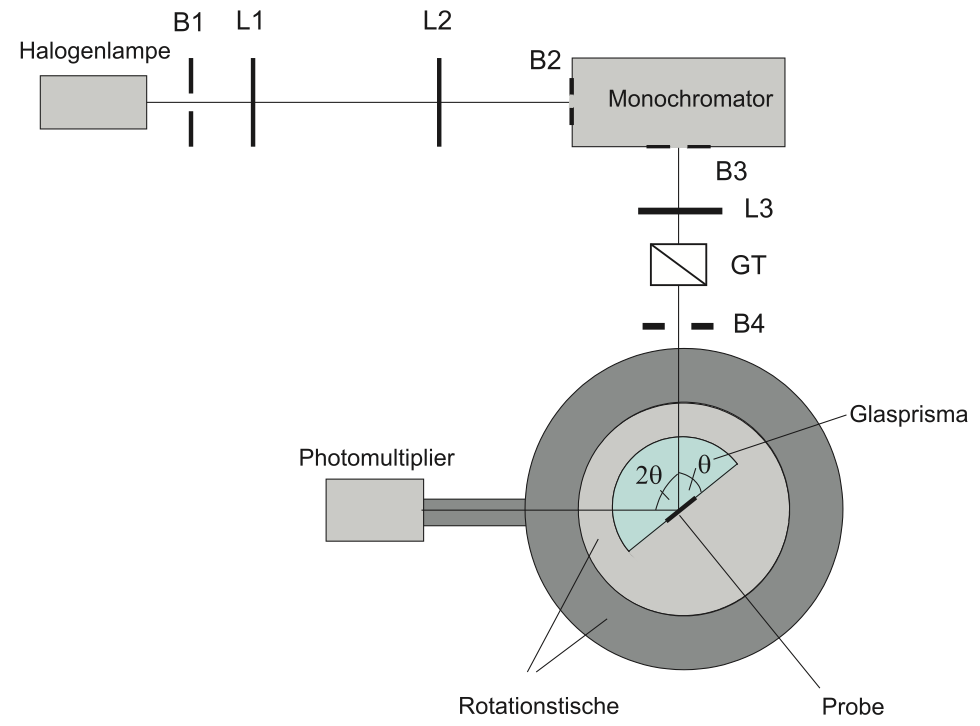
\includegraphics[width=1\textwidth]{op-aufbau.png}
	\caption{Aufbau zur Untersuchung der Oberfl�chenplasmonen}
	\label{fig:opaufbau}
\end{figure}
In diesem Versuch m�chten wir eine Probe mit $p$-polarisiertem monochromatischem
Licht bei variierendem Winkel bescheinen und dabei den Aufbau so konstruieren,
dass die Wellenl�nge des Lichtes als Parameter sich auch leicht �ndern l�sst. 

Dazu verwenden wir eine Halogenlampe, dessen Licht wir durch eine Blende und
zwei Linsen in einen Monochromator lenken. Die Lampe emittiert ein weites,
kontinuierliches Spektrum an Licht, dass im Monochromator auf ein Prisma trifft,
welches die Anteile des Lichts frequenzabh�ngig bricht.
Durch Drehung des Prismas k�nnen wir nun die Frequenz des Lichtes,
das aus einen Spalt wieder austritt, leicht variieren. 

Das Licht wird dann polarisiert und trifft auf das Glasprisma und die Probe,
wo es die Plasmonen anregen soll. Ein Teil des Lichtes wird auf einen Photomultiplier
reflektiert, wo seine Intensit�t gemessen wird. 

Die Probe ist zusammen mit dem Glasprisma und dem Photomultiplier auf einem
Rotationstisch befestigt. Diesen kann man manuell oder motorisiert bedienen
und damit den Winkel, mit dem das Licht auf die Probe und den Multiplier trifft,
abfahren.

Bevor wir mit der eigentlichen Untersuchung der Oberfl�chenplasmonen starten k�nnen,
m�ssen wir zuerst den Winkel des Rotationstisches kalibrieren.
Dazu nutzen wir den Effekt der Totalreflexion aus, indem wir den Aufbau
ohne Probe konstruieren und die Totalreflexion am �bergang Glasprisma-Luft
messen. Bei verschiedenen Wellenl�ngen gehen wir einen gro�en Winkelbereich
durch und vergleichen dann die berechneten theoretischen Werte mit den gemessenen
und verwenden die Differenz von nun an als Kalibrierungskonstante.

\section{Oberfl�chenplasmonen auf einer glatten Probe}

Im ersten Versuchsteil arbeiten wir mit Silber-Proben, die eine vorgegebene
Schichtdicke von 20nm--70nm haben. Im ersten Durchgang arbeiten wir mit Licht
der Wellenl�nge 550 nm und variieren bei festen Schichtdicken den Einfallswinkel
und messen die Reflektivit�t.
Durch einen Fit mit Mathematica k�nnen wir in
der Auswertung die angegebene Schichtdicke mehr oder weniger �berpr�fen.

Um die Dispersionsrelation der Oberfl�chenplasmonen zu bestimmen, nehmen wir die
Probe mit dem tiefsten Absorptionsprofil und fahren erneut bei verschiedenen
Wellenl�ngen den relevanten Winkelbereich durch.

\section{Oberfl�chenplasmonen auf einer gittermodulierten Probe}

Bei der Untersuchung der Probe mit in einer Richtung periodisch modulierter
Oberfl�che bestimmen wir zun�chst die Gr��e ihrer Gitterkonstanten.
Dazu nutzen wir die Interferenzeffekte unter der Beugung am Gitter aus.
Mit einem Laser bescheinen wir die Probe unter einem senkrechten Winkel und
messen den Winkel zwischen den Beugungsmaxima 0. und 1. Ordnung.

In der eigentlichen Messung verwenden wir die Gitter-Probe, wobei der �brige Aufbau
bis auf das Glasprisma, das nun nicht ben�tigt wird, gleich bleibt.
Zur Justage der Gitterprobe kann man die Beugungseffekte ausnutzen,
um die Richtung der Gitterperiodizit�t in die Ebene des Aufbaus einzustellen.

Wir w�hlen einen Messbereich von 475nm--625nm f�r die Wellenl�nge und variieren
jeweils wieder den Einfallswinkel und messen die Reflektivit�t.